%%%%%%%%%%%%%%%%%%%%%%%%%%%%%%%%%%%%%%%%%%%%%%%
%
%   Methodology
%
%%%%%%%%%%%%%%%%%%%%%%%%%%%%%%%%%%%%%%%%%%%%%%%
\section{Proposed Framework}
\label{ch5_methodology}

The proposed framework is graphically presented in Figure \ref{topology}. The training fold is reduced by AllKNN \cite{tomek1976} as an instance selection method to select representative samples. The selected data by AllKNN will be the source to build a group of heterogeneous classifiers. A pruning set is formed using stratified sampling with 70\% from the train. The pruning set will be the source to rank the individual classifiers during ensemble selection. Using this methodology, the following state-of-art ensembles will be trained for comparison purposes:

\begin{itemize}[nosep]
   \item[-] RFSM: Random Forest \cite{breiman2001} is learned from the selected data.
   \item[-] UNP: The proposed heterogeneous classifiers, Section (\ref{proposed.mcs}), without pruning  learned from the selected data.
   \item[-] RFCOM: Random Forest is learned from the whole training data.
   \item[-] SAMME: (Stagewise Additive Modeling
using a Multi-class Exponential loss function \cite{hastie2009}), which is trained from whole training data and extends the AdaBoost algorithm to the multiclass case.
\item[-] XGBoost: eXtreme Gradient Boosting decision tree \citep{chen2016} which is trained from the whole training data.
\vspace*{.3cm}

\end{itemize}
  \begin{figure*}[!ht]
\centering
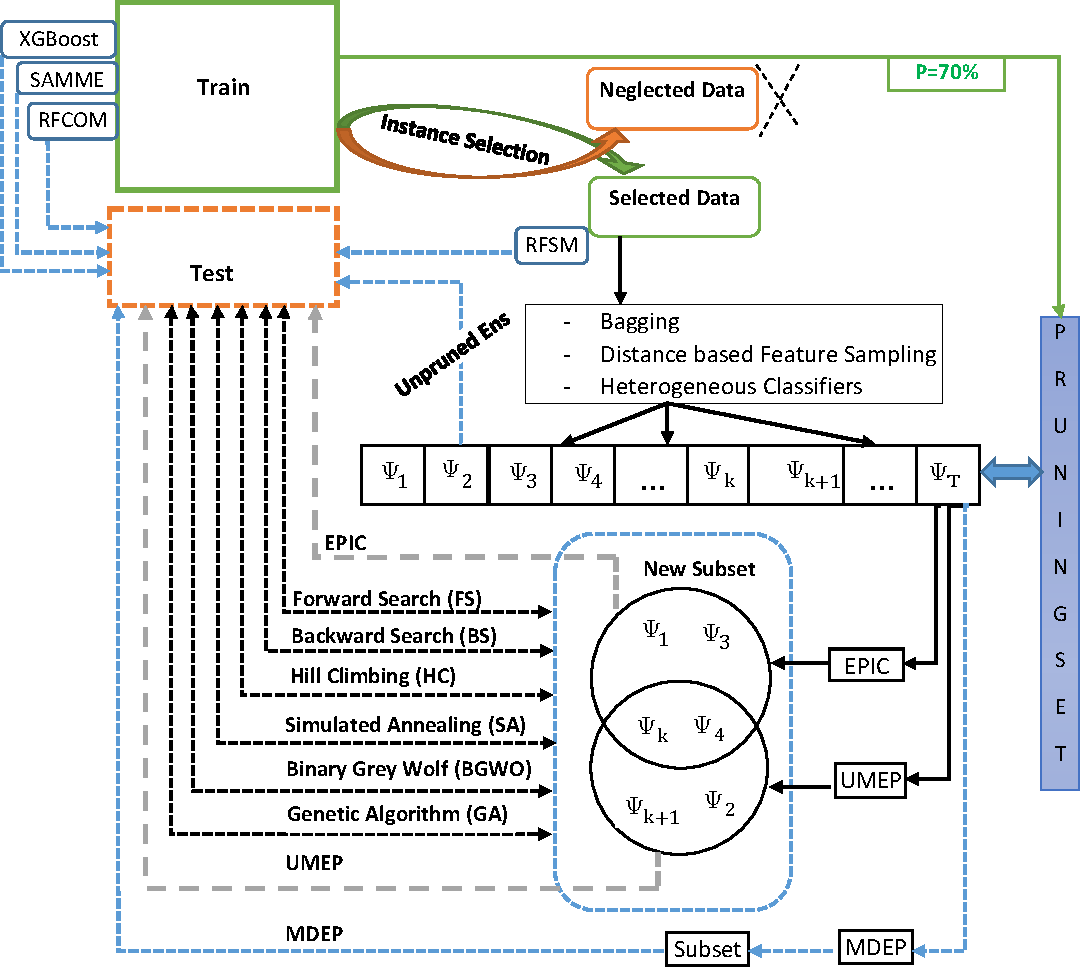
\includegraphics[width=.9\textwidth]{5_Guided_Search/fig/final-topology.pdf}
\caption{ The proposed ensemble selection in the presence of selected samples.}
\label{topology}
\end{figure*}


The two phases for cleaning noisy border samples, Section \ref{Training-set-selection}, and building heterogeneous MCS, Section \ref{proposed.mcs}, will not be changed. While we propose a guided search to prune the proposed ensemble. Therefore, we benefit from IS techniques and ensemble selection, rather than training large-size ensembles from large-size training data. 
   



\textbf{The Proposed Guided Search for Ensemble Pruning}: Having a large-size ensemble will limit the search capability of the well-known pruning metrics. As each pruning metric puts pressure to select a subset of classifiers with a specific property. For example, EPIC \cite{lu2010} concentrates on the classifier's diversity with the peer members. While UMEP \cite{guo2013} focuses more to select classifiers that behave well with low-margin samples. Regarding that, and with the large pool size of classifiers, the performance of the current pruning methods could vanish. Experimentally, Fig. \ref{conflicting} shows the generalized accuracy of the identified subensemble via different pruning methods, UMEP and EPIC, from different ensemble sizes. From Fig. \ref{conflicting}, we confirm that each metric is more important to a particular dataset. We conclude that paying no attention to other heuristic information affects the search process badly, and returns a subensemble with a limited accuracy.  

\vspace*{.3cm}
\begin{figure*}[h]
\begin{center}\scriptsize
  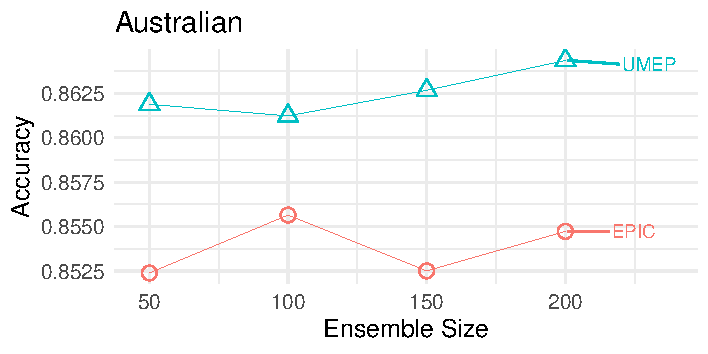
\includegraphics[width=.497\textwidth]{5_Guided_Search/fig/UMEP-EPIC-Australian.pdf}
  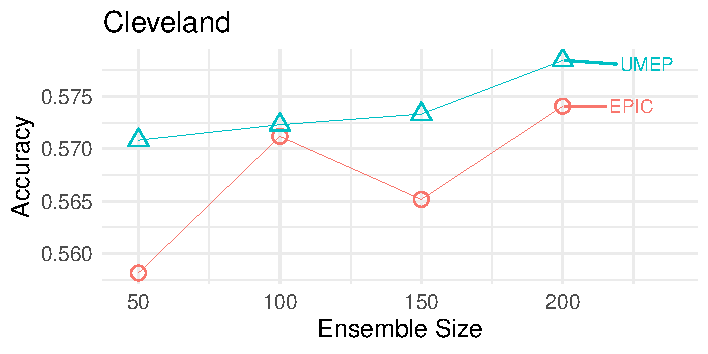
\includegraphics[width=.497\textwidth]{5_Guided_Search/fig/UMEP-EPIC-Cleveland.pdf}\\ 
  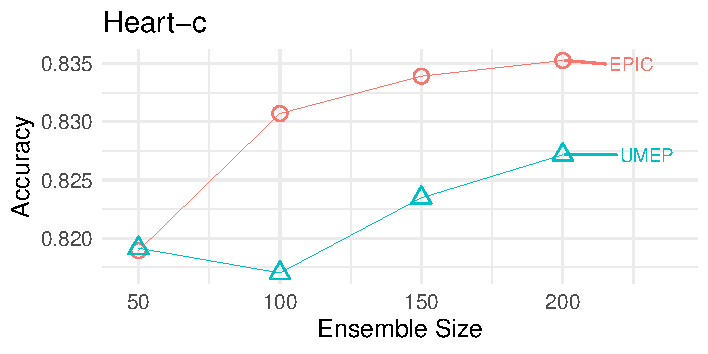
\includegraphics[width=.497\textwidth]{5_Guided_Search/fig/UMEP-EPIC-Heart-c.pdf}
   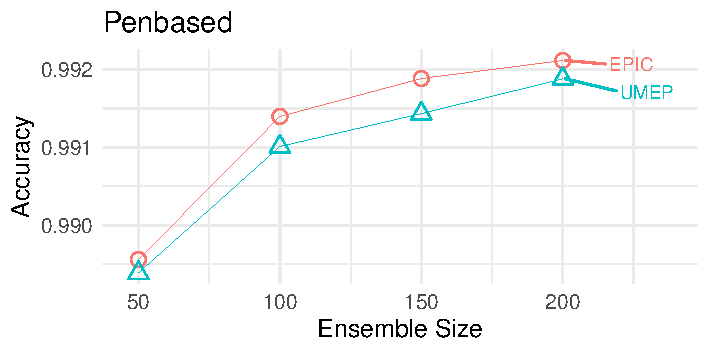
\includegraphics[width=.497\textwidth]{5_Guided_Search/fig/UMEP-EPIC-Penbased.pdf}\\
\end{center}
\caption{The conflict between both EPIC and UMEP, to be handled in this chapter.}
\label{conflicting}
\end{figure*}


Inspired by the above analysis, we can narrow the original search space by directing the search to promising areas. This is what EPIC and UMEP  return, each metric recommends a subspace according to their heuristic measures. Preferring one metric over the other will blinds a subspace that could contain crucial information. The two ordering-based pruning techniques, EPIC \cite{lu2010} and UMEP \cite{guo2013}, will be applied to determine the promising subspaces in advance. After that, the search process can be started. The details are as follows: 
 
 \begin{itemize}[nosep]
\item Each metric will rank the set of classifiers differently, but at least there will be common classifiers in-between.
 \item After ranking, a predetermined percentage, $P$, will be used to select a subset of classifiers. 
 \item A narrow space carrying the properties of both metrics will be formed via merging their output subsets, \textit{as in Fig. \ref{topology}}.
 \item The new subspace will be searched via Forward Search (FS) \footnote{Package Fselector:https://cran.r-project.org/web/packages/FSelector\label{fselect}}, Backward Search (BS)\textsuperscript{\ref{fselect}}, Hill Climbing (HC) \cite{cortez2014}, Simulated Annealing (SA) \cite{cortez2014}, Binary Grey Wolf Optimizer (BGWO) \cite{emary2016}, and Binary Genetic Algorithm (GA)\footnote{Package genalg:https://cran.r-project.org/web/packages/genalg}.    
 \end{itemize} 


Via guided search, we try to alleviate the randomness of the search process that could increase with large-size ensembles. To the best of our knowledge, this work is the first to handle the conflict between EPIC and UMEP. Moreover, it can be categorized as ensembling the pruning metrics themselves to get better performance than each of them.